\documentclass[12pt]{letter}

\usepackage{tikz,amsmath,amssymb}
\usetikzlibrary{external,arrows,decorations.pathmorphing,decorations.markings,backgrounds,positioning,fit,petri,decorations.pathreplacing,positioning}
\tikzexternalize

\begin{document}

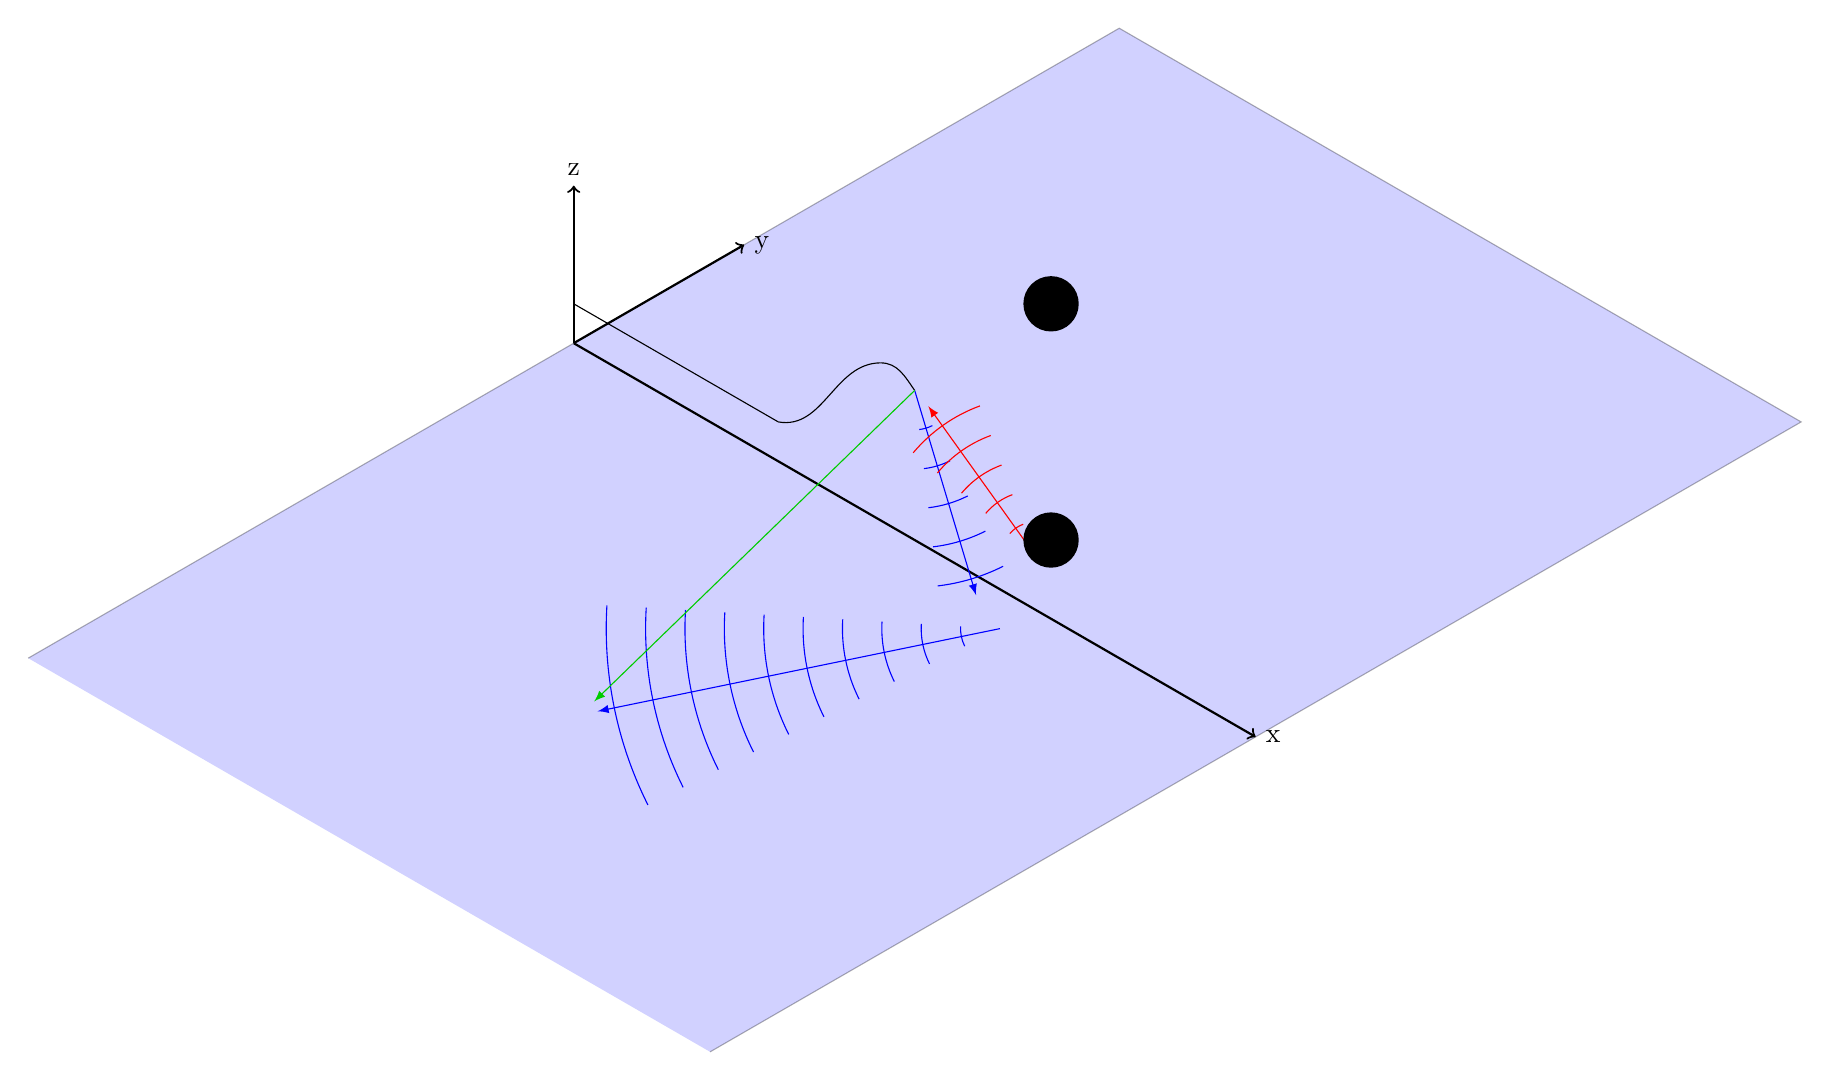
\begin{tikzpicture}[x={(0.866cm,-0.5cm)}, y={(0.866cm,0.5cm)}, z={(0cm,1cm)}, scale=1.0,
    axis/.style={thick,->},
    surfacePlane/.style={fill=blue!60!white, opacity=0.3},
  ]

    % Colors
    \colorlet{darkgreen}{green!50!black}
    \colorlet{lightgreen}{green!80!black}
    \colorlet{darkred}{red!50!black}
    \colorlet{lightred}{red!80!black}

 
    \coordinate (O) at (0, 0, 0);
    \coordinate (T) at (4, 3, 1);
    \coordinate (R) at (8, -1, 2);
    \coordinate (P) at (7, 0, 0);
    \coordinate (m1) at (5,0,1.9);
    \coordinate (m2) at (5,-5,0.25);
    \coordinate (m3) at (4.75,-4.75,0.25);
    \coordinate (m4) at (5.25,-5.25,0.25);

    %draw the surface
    \filldraw[surfacePlane] (0,-8,0) -- (0,8,0) -- (10,8,0) -- (10,-8,0);

    %draw the axis
    \draw[axis] (O) -- +(10, 0,   0) node [right] {x};
    \draw[axis] (O) -- +(0,  2.5, 0) node [right] {y};
    \draw[axis] (O) -- +(0,  0,   2) node [above] {z};

    %draw the illuminator path
    \draw[] (0,0,0.5) -- (3,0,0.5);
    \draw[] (3,0,0.5) to [out=-10,in=180] (4.5,0,2);
    \draw[] (4.5,0,2) to [out=0,in=125] (m1);

    %draw the missile paths
    %\draw[] (4,-7,0.25) -- (m2);
    %\draw[] (3.75,-6.75,0.25) -- (m3);
    %\draw[] (4.25,-7.25,0.25) -- (m4);
   
    %wave from illuminator to ship
    \draw[-latex,blue] (5,0,1.9) -- (6.3, -0.4, 0.15);
    \draw[blue,decorate,decoration={expanding waves, segment length = 5mm, angle=10}] (5,0,1.9) -- (6.3, -0.4, 0.15)(6.75,-0.5,0);

    %wave from ship to salvo
    \draw[-latex,blue] (6.75,-0.5,0) -- (5.1,-4.75,0.25);
    \draw[blue,decorate,decoration={expanding waves, segment length = 5mm, angle=15}]  (6.75,-0.5,0) -- (5.1,-4.75,0.25);

    %wave from ship to illuminator (EA)
    \draw[-latex,red] (6.85,-0.1,0.8) --  (5.3,-0.1,1.9);
    \draw[red,decorate,decoration={expanding waves, segment length = 4mm, angle=15}] (6.85,-0.1,0.8) --  (5.35,-0.1,1.9);

    %wave from ship to salvo (Data link)
    \draw[-latex,lightgreen] (m1) to (5.2,-4.9,0.5);
    
    \fill (T) circle (10pt);
    
    \fill (R) circle (10pt);


    %%add the images
    %add the ship image
    %\node (ship) at (P)
        %{\includegraphics[width=0.25\textwidth]{glow.png}};

    %add the illuminator image
    %\node[rotate=125,transform shape] at (m1)
       %{\includegraphics[width=0.5cm]{m1.png}};

    %add the 1st missile image
    %\node[rotate=190,transform shape] at (m2)
      %{\includegraphics[width=0.5cm]{m2.png}};

    %add the 2nd missile image
    %\node[rotate=190,transform shape] at (m3)
           %{\includegraphics[width=0.5cm]{m3.png}};

    %add the 3rd  missile image
    %\node[rotate=190,transform shape] at (m4)
      %{\includegraphics[width=0.5cm]{m4.png}};

    %%add the text boxes
  %  \draw (8.8,0.7,1) node [font=\tiny,draw,fill=white, text width=2.25cm, text centered]{Adversary Surface Action Group};

   % \draw (3.75,-5.25,0.75) node [font=\tiny,draw,fill=white,text width=2cm, text centered]{Heterogeneous salvo with passive sensing};

    %\draw (3.7,1.85,1.1) node [font=\tiny,draw,fill=white,text width=2cm, text centered]{Stand-off Illuminator};

    %\draw (4.25,-1.75,0.25) node [font=\tiny,draw,fill=white,text width=2cm, text centered]{Potential Data Link};

    %\coordinate (MS) at (7.7,-5.6,0.25);
    %\draw[->,dashed] (MS) -- (6.5,-4,0);
    %\draw (MS) node [font=\tiny,draw,fill=white,text width=2cm, text centered]{Multistatic Signal};

    %\coordinate (EA) at (6.25,3,0.25);
   % \draw[->,dashed] (EA) -- (5.75,0.5,1);
   % \draw (EA) node [font=\tiny,draw,fill=white,text width=2.5cm, text centered]{EA directed \underline{AWAY} from weapons};
    
\end{tikzpicture}

\end{document}
